\begin{ccRefConcept}{TriangulationDataStructure}

\ccDefinition

The \ccRefName\ concept describes objects responsible for storing and
maintaining the combinatorial part of a
$d$-dimensional pure simplicial complex. Its topology is the topology
of the sphere  $\sphere^d$ with $d\in[-2,D]$
or possibly of another $d$-dimensional manifold without boundary 
(that can be embedded in an higher dimension).
 In a  pure (or homogeneous) simplicial $d$-complex, all
 faces are sub-faces of some $d$-simplex. (A
simplex is also a face of itself.) In particular, it does not
contain any $d+1$-face, and any $d-1$-face belongs to exactly
two $d$-simensional {\em full cell}. 

Values of $d$ (the \emph{current dimension} of the complex) include \begin{itemize}

\item[-2] This corresponds to the non-existence of any object in
$\sphere^D.$

\item[-1] This corresponds to a single vertex and a single simplex. In a
geometric realization of the \ccRefName\ (\emph{e.g.}, in a
\ccc{Triangulation<TrTraits, TDS>} or a
\ccc{Delaunay_triangulation<TrTraits, TDS>}), this vertex
corresponds to \emph{the vertex at infinity}.

\item[0] This corresponds to two vertices, each adjacent to one $0$-simplex;
the two simplices being neighbor of each other. This is the unique
triangulation of the $0$-sphere.

\item[$d>0$] This corresponds to a standard triangulation of the sphere
$\sphere^d$.
\end{itemize}

An $i$-simplex is a simplex with $i+1$ vertices. An $i$-simplex $\sigma$ is
\textbf{incident} to a $j$-simplex $\sigma'$, $j<i$, if and only if $\sigma'$
is a proper face of $\sigma$. 
%Two simplices are \textbf{adjacent} if the
%intersection of their vertex-set is not empty.

\ccHasModels

\ccc{Triangulation_data_structure<Dimensionality, TDSVertex, TDSSimplex>}

\ccTypes

\ccNestedType{Vertex}
{
A model of the concept \ccc{TriangulationDSVertex}.
}
\ccGlue
\ccNestedType{Simplex}
{
A model of the concept \ccc{TriangulationDSSimplex}.
}

The concept \ccRefName\ also defines a type for describing facets of the
triangulation with codimension~1:

\ccTypedef{typedef std::pair<Full_cell_handle, int> Facet;}
{A facet of a full cell. Its dimension is
\ccc{current_dimension()-1}. \ccc{Facet f(c,i)} represents the facet of
full cell \ccc{c} opposite to its \ccc{i}-th vertex}

\ccNestedType{Face}
{A model of the concept \ccc{TriangulationFace}.}

Vertices and simplices are manipulated via \emph{handles}. Handles support the
usual two dereference operators \ccc{operator*} and \ccc{operator->}.

\ccNestedType{Vertex_handle}
{
Handle to a \ccc{Vertex}.
}
%\ccGlue
%\ccNestedType{Vertex_const_handle}
%{
%Handle to a \ccc{const Vertex}.
%}
\ccGlue
\ccNestedType{Full_cell_handle}
{
Handle to a \ccc{Full_cell}.
}
%\ccGlue
%\ccNestedType{Full_cell_const_handle}
%{
%Handle to a \ccc{const Full_cell}.
%}

Vertices, facets and cells can be iterated over using \emph{iterators}.
Iterators support the usual two dereference operators \ccc{operator*} and
\ccc{operator->}.

\ccNestedType{Vertex_iterator}
{
Iterator over the list of vertices.
}
%\ccGlue
%\ccNestedType{Vertex_const_iterator}
%{
%Iterator over the list of vertices (\ccc{const} casted).
%}
\ccGlue
\ccNestedType{Full _cell_iterator}
{
Iterator over the list of cells.
}
%\ccGlue
%\ccNestedType{Simplex_const_iterator}
%{
%Iterator over the list of simplices (\ccc{const} casted).
%}
\ccGlue
\ccNestedType{Facet_iterator}
{
Iterator over the facets of the complex.
}

\ccNestedType{size_type}{Size type (an unsigned integral type)}
\ccNestedType{difference_type}{Difference type (a signed integral type)}

\ccCreation
\ccCreationVariable{tds}

\ccConstructor{Triangulation(const int dim);} { Creates an instance \ccVar\ of
type \ccRefName. The maximal dimension of its cells is \ccc{dim} and
\ccVar\ is initialized to the empty triangulation. Thus,
\ccVar.\ccc{current_dimension()} equals \ccc{-2}.}

%\ccOperations

\ccHeading{Queries}	% --------------------------------------------- QUERIES

\ccMethod{int ambient_dimension() const;} { Returns the maximal dimension of
the cells that can be stored in the triangulation \ccVar. \ccPostcond the
returned value is positive. }

\ccMethod{int current_dimension() const;} { Returns the dimension of the
full dimensional cells stored in the triangulation. It holds that
\ccVar.\ccc{current_dimension()=-2} if and only if \ccVar.\ccc{empty()} is
\ccc{true}. \ccPostcond the returned value \ccc{d} satisfies 
$-2\leq d \leq$\ccVar.\ccc{ambient_dimension()}. }

\ccMethod{bool empty() const;} { Returns \ccc{true} if the regular complex
contains no simplex. Returns \ccc{false} otherwise. }

\ccMethod{size_type number_of_vertices() const;}
{Returns the number of vertices stored in the regular complex.}

\ccMethod{size_type number_of_full_cells() const;}
{Returns the number of cells stored in the regular complex.}

\ccMethod{bool is_vertex(const Vertex_handle & v) const;}
{}

\ccMethod{bool is_full_cell(const Full_cell_handle & c) const;}
{}

\ccMethod{template< typename TraversalPredicate, typename OutputIterator >
void gather_full_cells(Full_cell_handle c, TraversalPredicate & tp,
OutputIterator & out) const;}
{This function computes (\emph{gathers}) a connected set of full cells
satifying a common criteria. Call them \emph{good} cells. It is assumed
that the argument \ccc{c} is a good cell. The cells are then
recursively explored by examining if, from a given good cell, its neighboring
cells are also good.\\
The argument \ccc{tp} is a predicate that takes as argument a \ccc{Facet}
whose containing \ccc{Full_cell} is good. The predicate must return \ccc{true}
if the traversal of that \ccc{Facet} leads to a good cell.\\
All the good cells are outputed into the last argument \ccc{out}.}

\ccMethod{template< typename OutputIterator > OutputIterator
incident_full_cells(Vertex_const_handle v, OutputIterator out) const;}
{Insert in \ccc{out} all the cells that are incident to the vertex
\ccc{v}, \emph{i.e.}, the full cells that have the \ccc{Vertex v} as a vertex.
Returns the (modified) output iterator.
\ccPrecond\ccc{is_full_cell(f.full_cell())}.}

\ccMethod{template< typename OutputIterator > OutputIterator
incident_full_cells(const Face & f, OutputIterator out) const;}
{Insert in \ccc{out} all the cells that are incident to the face \ccc{f},
\emph{i.e.}, the full cells that have the \ccc{Face f} as a subface.
Returns the (probably modified) output iterator.
\ccPrecond\ccc{is_full_cell(f.full_cell())}.}

\ccMethod{template< typename OutputIterator > OutputIterator
compute_star(const Face & f, OutputIterator out) const;}
{Insert in \ccc{out} all the full cells that share at least one vertex with the \ccc{Face
f}. Returns the (probably modified) output iterator.
\ccPrecond\ccc{is_full_cell(f.full_cell())}.}

% \ccMethod{template< typename OutputIterator > OutputIterator
% gather_incident_faces(Vertex_const_handle v, const int d, OutputIterator
% out);}{Constructs all the \ccc{Face}s of dimension \ccc{d} incident to
% \ccc{Vertex} v and inserts them in the \ccc{OutputIterator out}.  If \ccc{d
% >=} \ccVar.\ccc{current_dimension()}, then no \ccc{Face} is
% constructed.\ccPrecond\ccc{0 < d}.}

% \ccMethod{template< typename OutputIterator > OutputIterator
% gather_incident_upper_faces(Vertex_const_handle v, const int d, OutputIterator
% out);}{Constructs all the \textbf{upper} \ccc{Face}s of dimension \ccc{d}
% incident to \ccc{Vertex} v and inserts them in the \ccc{OutputIterator out}.\\
% Assuming some total ordering on the vertices of the complex (which is
% invariant as long as no vertex is inserted in or removed from the complex), a
% \ccc{Face} incident to \ccc{v} is an \emph{upper} \ccc{Face} if and only if
% its vertices occur at \ccc{v} or beyond \ccc{v} in the ordering.\\ In
% particular, taking the disjoint union of the upper \ccc{Face}s of dimension
% \ccc{d} incident to every vertex of the complex yields exactly the set of
% faces of dimension \ccc{d} of the complex.\\ The constructed \ccc{Faces} are
% lexicographically ordered (using the vertex order as base ordering). If \ccc{d
% >=} \ccVar.\ccc{current_dimension()}, then no \ccc{Face} is
% constructed.\ccPrecond\ccc{0 < d}.}

% \ccGlue\ccMethod{template< typename OutputIterator, typename Comparator >
% OutputIterator gather_incident_upper_faces(Vertex_const_handle v, const int d,
% OutputIterator out, Comparator cmp);} {Same as above, but uses \ccc{cmp} as
% the vertex ordering to define the upper faces.}

\ccHeading{Accessing the vertices} % --------------------- ACCESS TO VERTICES

\ccMethod{Vertex_handle vertex(Full_cell_handle c, const int i) const;}%{}
%\ccGlue
%\ccMethod{Vertex_const_handle vertex(Full_cell_const_handle c, const int i) const;}
{ Returns a handle to the \ccc{i}-th \ccc{Vertex} of the \ccc{Full_cell} \ccc{c}.
\ccPrecond \ccc{0 <= i <=} \ccVar.\ccc{current_dimension()}.}

\ccMethod{int mirror_index(Full_cell_handle c, int i) const;}%{}
%\ccGlue\ccMethod{int mirror_index(Full_cell_const_handle s, int i) const;}
{Returns the index of the vertex mirror of the \ccc{i}-th vertex of \ccc{c}.
Equivalently, returns the index of \ccc{s} in its \ccc{i}-th neighbor.
\note{If there is no \ccc{i}-th neighbor of \ccc{c}, then
returns \ccc{-1}. OD: c'est quoi ca ? il y a toujours un i$i$th neighbor
si $d<D$.}
\ccPrecond \ccc{0 <= i <=} \ccVar.\ccc{current_dimension}()\\
and \ccc{s != Simplex_handle()}. }

%\ccMethod{Vertex_const_iterator vertices_begin() const;}
%{
%}
%\ccGlue
\ccMethod{Vertex_iterator vertices_begin();}
{
The first vertex of \ccVar.
}
%\ccGlue
%\ccMethod{Vertex_const_iterator vertices_end() const;}
%{
%}
\ccGlue
\ccMethod{Vertex_iterator vertices_end();}
{
The beyond vertex of \ccVar.
}

\ccHeading{Accessing the full cells} % ------------------- ACCESS TO CELLS

\ccMethod{Full_cell_handle full_cell(Vertex_handle v) const;}%{}
%\ccGlue
%\ccMethod{Full_cell_const_handle simplex(Vertex_const_handle v) const;}
{Returns a full cell incident to \ccc{Vertex} \ccc{v}. Note that this simplex is
not unique (\ccc{v} is typically adjacent to more than one simplex).
\ccPrecond\ccc{v != Vertex_handle()}}

\ccMethod{Full_cell_handle neighbor(Full_cell_handle c, int i) const;}%{}
%\ccGlue
%\ccMethod{Full_cell_const_handle neighbor(Full_cell_const_handle s, int i) const;} 
{ Returns a \ccc{Full_cell_handle} pointing to the \ccc{Full_cell}
opposite to the \ccc{i}-th vertex of \ccc{s}. 
\note{If there is no opposite cell,
then returns \ccc{Full_cell_handle()}.OD: meme rq}
\ccPrecond\ccc{0 <= i <=}\ccVar.\ccc{current_dimension()}\\
and \ccc{c != Full_cell_handle()}}

%\ccMethod{Simplex_const_iterator full_cells_begin() const;}
%{
%}
%\ccGlue
\ccMethod{Full_cell_iterator full_cells_begin();}
{
The first full cell of \ccVar.
}
%\ccGlue
%\ccMethod{Simplex_const_iterator full_cells_end() const;}
%{
%}
\ccGlue
\ccMethod{Full_cell_iterator full_cells_end();}
{
The beyond full cell of \ccVar.
}

\ccHeading{Faces and Facets} % - - - - - - - - - - - - - - - - - - - - FACETS

\ccMethod{Facet_iterator facets_begin();}
{Iterator to the first facet of the triangulation.}
\ccGlue
\ccMethod{Facet_iterator facets_end();}
{Iterator to the beyond facet of the triangulation.}

\ccMethod{Full_cell_handle full_cell_of(const Facet & f) const;}
{Returns a full cell containing the facet \ccc{f}}

\ccMethod{int index_of_covertex(const Facet & f) const;}
{Returns the index of vertex of the cell \ccc{c=}\ccVar.\ccc{full_cell_of(f)}
which does \textbf{not} belong to \ccc{c}.}

\ccMethod{Face make_empty_face() const;}{Returns an empty \ccc{Face}.}

\begin{ccAdvanced}

\ccMethod{bool is_boundary_facet(const Facet & f) const;}
{When a subset of the full cells has their \ccc{flags} set to \ccc{1}, this
function returns \ccc{true} when the \ccc{Facet f} is part of the boundary of
that subset, and \ccc{false} otherwise.
\note{bof, ces trucs de flags sont publics ? si oui ils faut qu'ils
  soient robustes et documenté partout}
}

\end{ccAdvanced}

\ccHeading{Vertex removal} % - - - - - - - - - - - - - - - - - - - - REMOVALS

\ccMethod{void clear();}
{Reinitializes \ccVar\ to the empty complex.}

\ccMethod{Vertex_handle collapse_face(const Face & f);} {Contracts the
\ccc{Face f} to a single vertex. Returns a handle to that vertex. \ccPrecond
The contracted triangulation must be valid (\emph{i.e.}, be a triangulation of
a sphere of dimension \ccVar.\ccc{current_dimension()}).}

\ccMethod{void remove_decrease_dimension(Vertex_handle v, Vertex_handle
star);} {This method does exactly the opposite of
\ccc{insert_increase_dimension()}. \ccPrecond Both vertices \ccc{v} and
\ccc{star} must share an edge with all vertices.
\ccc{current_dimension() >= -1}.}

\begin{ccAdvanced}

\ccMethod{void delete_vertex(Vertex_handle v);}
{Remove the vertex \ccc{v} from the triangulation. This does not take care of
erasing the references to \ccc{v} in other parts of the triangulation.}

\ccMethod{void delete_full_cell(Full_cell_handle c);}
{Remove the cell \ccc{c} from the triangulation. This does not take care of
erasing the references to \ccc{c} in other parts of the triangulation.}

\ccMethod{template< typename ForwardIterator > void
    delete_full_cells(ForwardIterator start, ForwardIterator end);}
{Remove the cells in the range \ccc{[start,end)} from the triangulation.
This does not take care of erasing the references to these cells in other parts of
the triangulation.}

\end{ccAdvanced}

\ccHeading{Vertex insertion} % - - - - - - - - - - - - - - - - - - INSERTIONS

\ccMethod{Vertex_handle insert_in_full_cell(Full_cell_handle c);}{Inserts a new
vertex \ccc{v} in the cell \ccc{c} and returns a handle to it. The cell
\ccc{c} is subdivided into \ccVar.\ccc{current_dimension())+1} cells which
share the vertex \ccc{v}.
\ccPrecond\ccc{0 <} \ccVar.\ccc{current_dimension()}\\ and
\ccc{c!=Simplex_handle()}\\ and \ccc{c} is a simplex of \ccVar.}
\begin{ccTexOnly}
\begin{center}
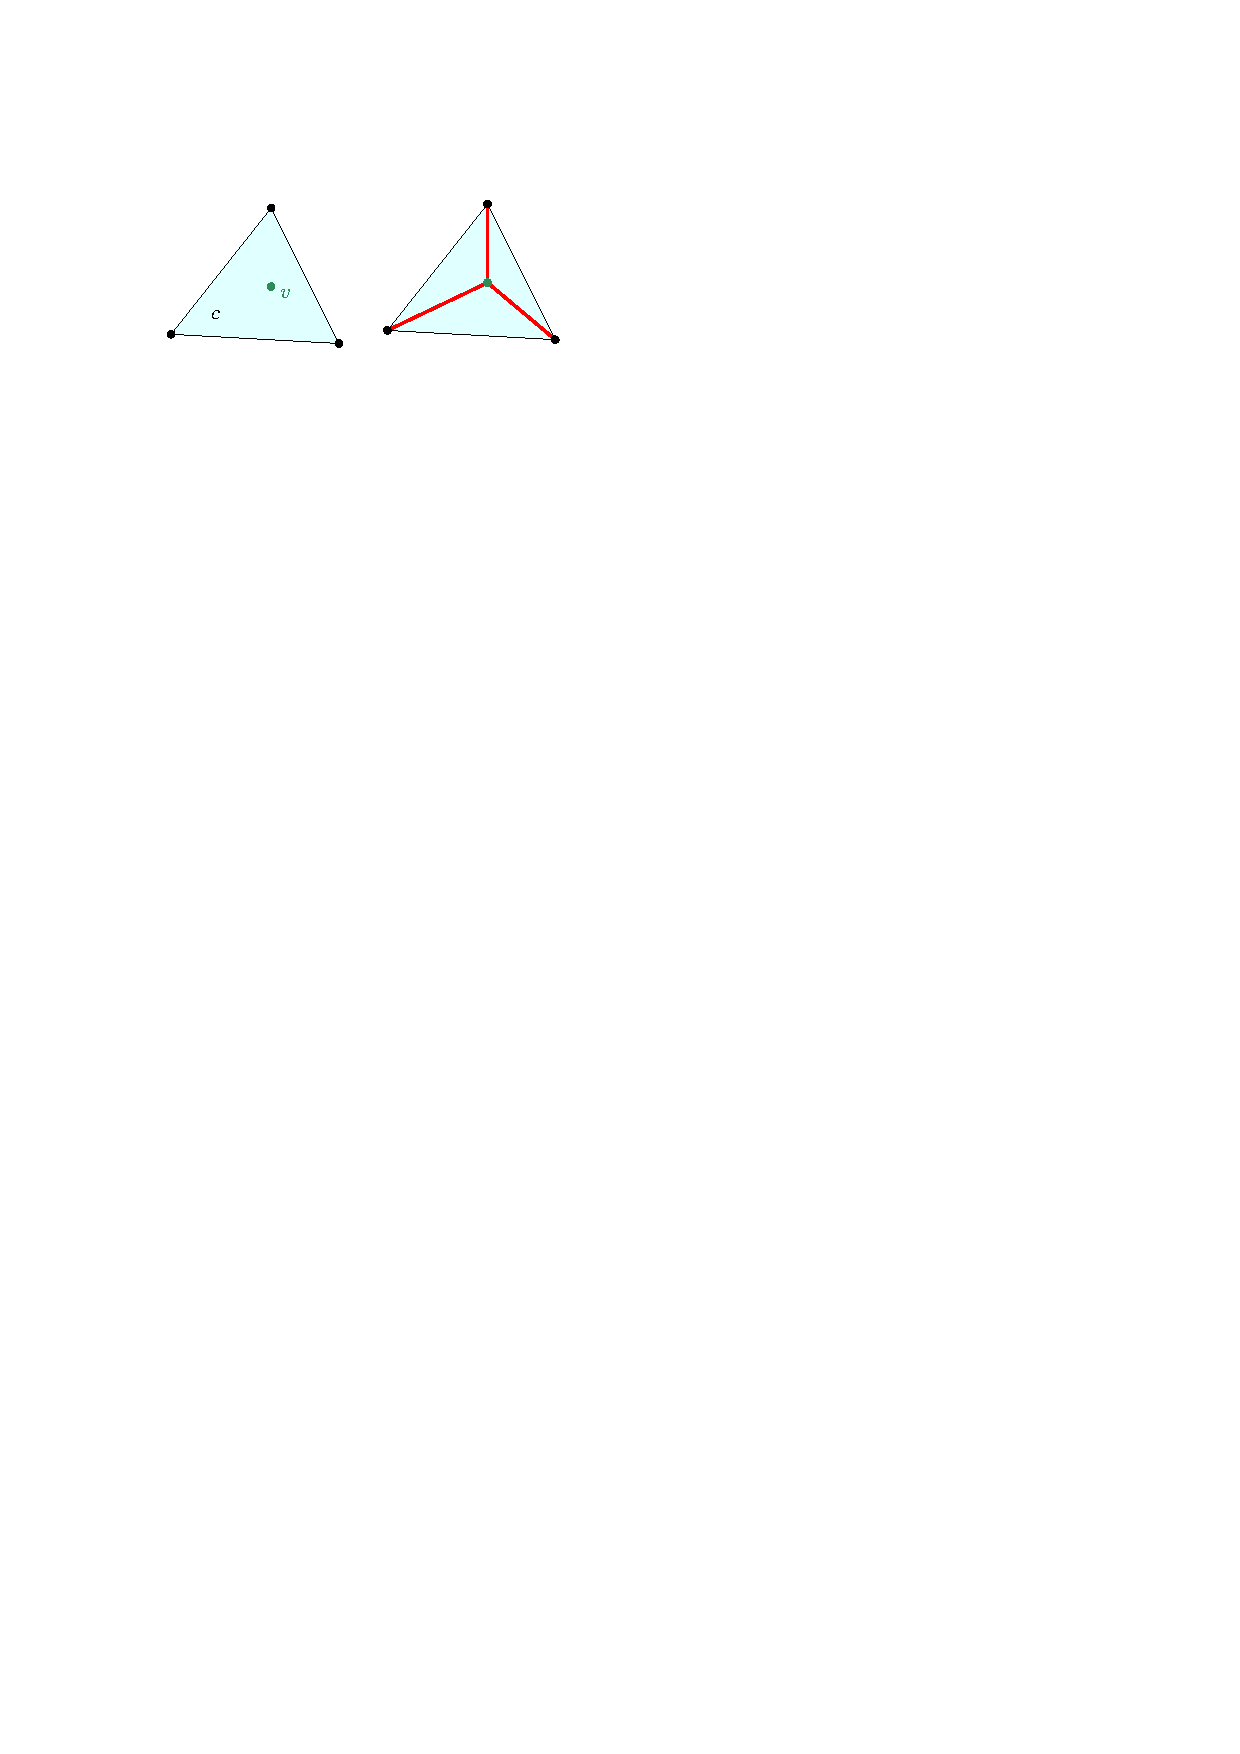
\includegraphics{Triangulation_ref/fig/insert-in-cell.pdf}
\end{center}
\end{ccTexOnly}
\begin{ccHtmlOnly}
<center>
<img border=0 src="./fig/insert-in-cell.png" align="middle" alt="The effect of insert_in_simplex()">
</center>
\end{ccHtmlOnly}

\ccMethod{Vertex_handle insert_in_face(const Face & f);}
{Inserts a vertex in the triangulation data structure by subdividing the
\ccc{Face f}. Returns a handle to the newly created \ccc{Vertex}.}
\begin{ccTexOnly}
\begin{center}
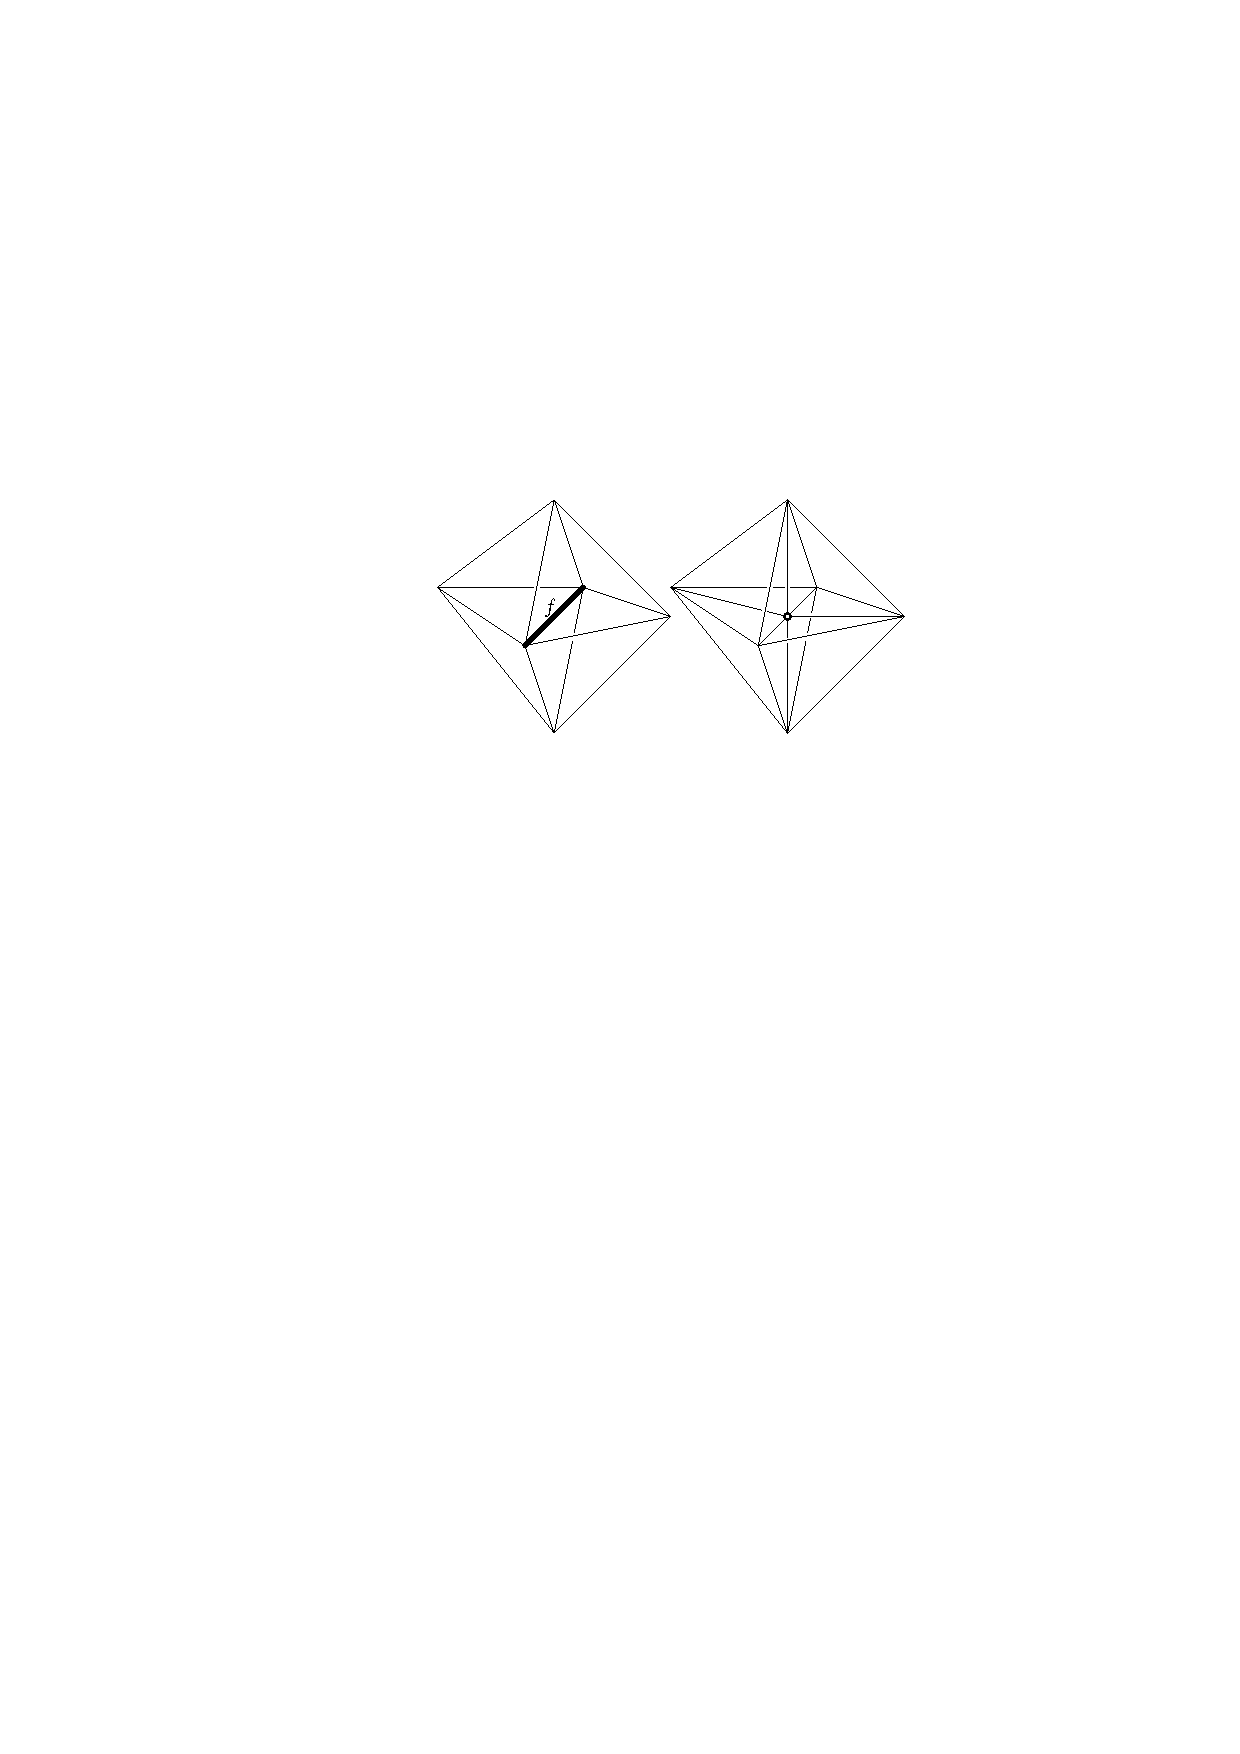
\includegraphics{Triangulation_ref/fig/insert-in-face.pdf}
\end{center}
\end{ccTexOnly}
\begin{ccHtmlOnly}
<center>
<img border=0 src="./fig/insert-in-face.png" align="middle" alt="The effect of insert_in_face()">
</center>
\end{ccHtmlOnly}

\ccMethod{Vertex_handle insert_in_facet(const Facet & ft);}
{Inserts a vertex in the triangulation data structure by subdividing the
\ccc{Facet ft}. Returns a handle to the newly created \ccc{Vertex}.}

\ccMethod{template< class ForwardIterator > Vertex_handle
insert_in_hole(ForwardIterator start, ForwardIterator end, Facet f);}{The
simplices in the range $C=$\ccc{[start, end)} are removed, thus forming a hole.
A \ccc{Vertex} is inserted and connected to the boundary of the hole in order
to ``close it''. A \ccc{Vertex_handle} to the new \ccc{Vertex} is returned.
\ccPrecond $C$ must be a (combinatorial) ball and not contain any vertex
all of whose adjacent simplices are in $C$. (This implies that
\ccVar.\ccc{current_dimension()}$\geq2$ if $|C|>1$.)\\ The boundary of
$C$ must be a (combinatorial) triangulation of the sphere
$\sphere^{d-1}$.}
\ccGlue
\ccMethod{template< class ForwardIterator, class OutputIterator >
Vertex_handle insert_in_hole(ForwardIterator start, ForwardIterator end, Facet
f, OutputIterator out);}{Same as above, but handles to the new simplices are
appended to the \ccc{out} output iterator.}

\ccMethod{Vertex_handle insert_increase_dimension(Vertex_handle star);}
{Transforms a triangulation of  the sphere $\sphere^d$ into the
triangulation of the sphere $\sphere^{d+1}$ by adding a new vertex \ccc{v}:
\ccc{v} is added to all simplices that do not contain the vertex \ccc{star} so
as to triangulate one of the two half-spheres of $\sphere^{d+1}$. The vertex
\ccc{star} already does triangulate the second half-sphere. (When there is an
associated geometric triangulation, \ccc{star} is in fact the vertex
associated with its infinite vertex.) The storage of the vertices in the
full cell is such that, if \ccc{f} was a cell of maximal dimension in the
initial complex, then \ccc{(f,v)}, in this order, is the corresponding cell
in the updated triangulation. A handle to \ccc{v} is returned.
\ccPrecond\ccVar.\ccc{current_dimension() < }
\ccVar.\ccc{ambient_dimension()} and \ccc{is_vertex(star)}}

\begin{ccAdvanced}

The following methods may destroy the integrity %(the ``purity'', one may say)
of the data structure. They are used internally. Use at your own risks.

\ccMethod{Full_cell_handle new_full_cell();} {Adds a new cell to \ccVar\ and
returns a handle to it. The new cell has no vertex and no neighbor yet.}

\ccMethod{Vertex_handle new_vertex();}
{Adds a new vertex to \ccVar\ and returns a handle to it. The new vertex has
no associated cell nor index yet.}

\ccMethod{void associate_vertex_with_full_cell(Full_cell_handle c, int i,
Vertex_handle v);}
{Sets the \ccc{i}-th vertex of \ccc{c} to \ccc{v} and, if \ccc{v} is non-NULL,
sets \ccc{c} as the adjacent cell of \ccc{v}.}

\ccMethod{void set_neighbors(Full_cell_handle ci, int i, Full_cell_handle cj, int
j);}
{Sets the neighbor opposite to vertex \ccc{i} of \ccc{Full_cell} \ccc{ci} to
\ccc{cj}. Sets the neighbor opposite to vertex \ccc{j} of \ccc{Full_cell}
\ccc{cj} to \ccc{ci}.}

\ccMethod{void set_current_dimension(int d);} { Forces the current dimension
of the complex to \ccc{d}. This will have weird consequences if you don't know
what you are doing. \ccPrecond \ccc{-1 <= d &&
d <=} \ccVar.\ccc{ambient_dimension()}}

\ccMethod{template< OutputIterator > Full_cell_handle insert_in_tagged_hole(
        Vertex_handle v, Facet f, OutputIterator new_simplices);}
{A set \ccc{C} of simplices satisfying the same condition as in method
\ccRefName\ccc{::insert_in_hole()} is assumed to be flagged to \ccc{1}. This
method creates new simplices from \ccc{Vertex} v to the boundary of \ccc{C}.
The boundary is recognized by checking the flags of the simplices.
This method is called by \ccRefName\ccc{::insert_in_hole()}.}

\end{ccAdvanced}

\ccHeading{Validity check} % - - - - - - - - - - - - - - - - - - - - VALIDITY

\ccMethod{bool is_valid(bool verbose = true, int level = 0) const;}
{Partially checks whether \ccVar\ is a triangulation. This function
returns \ccc{true} if each vertex is a vertex of the cell of which it
claims to be a vertex, if the vertices of every cell are pairwise distinct,
if the neighbor relationship is symmetric, and if neighboring cells share
exactly \ccVar.\ccc{current_dimension()} vertices. It prints an error message
if one of these conditions is violated and the \ccc{verbose} parameter is
\ccc{true}. Passing these tests does not garanty that we have a
triangulation (abstract pure
complex). In particular, for example, it is not
checked whether cells that share \ccVar.\ccc{current_dimension()} vertices
are neighbors in the data structure.}

\ccHeading{Input/Output}

\ccFunction{istream & operator>>(istream & is, TriangulationDataStructure &
tds);}
{Reads a combinatorial triangulation from \ccc{is} and assigns it to
\ccc{tds}. \ccPrecond The dimension of the input complex must be less than or
equal to \ccc{pcds.ambient_dimension()}.}

\ccFunction{ostream & operator<<(ostream & os, const TriangulationDataStructure
& tds);}
{Writes \ccc{tds} into the stream \ccc{os}}

The information stored in the \ccc{iostream} is: the current dimension (which
must be \ccc{<=} \ccVar.\ccc{ambient_dimension()}), the number of vertices,
the number of cells, the indices of the vertices of each cell and then the
indices of the neighbors of each cell, where the index corresponds to the
preceding list of cells.

TODO: explain that custom vertex/cell type will have their data input and
output properly (if the classes provide these operators).

\ccSeeAlso

\ccc{TriangulationDSVertex}\\
\ccc{TriangulationDSSimplex}

\end{ccRefConcept}
